\documentclass[aspectratio=169]{beamer}
\usepackage[framemethod=tikz]{mdframed}
\usepackage{pgfplots}
\usepackage{tikz}
\usepackage{url}
\usepackage{xcolor}
\usepackage{xmpmulti}
\usetikzlibrary{shapes,arrows}
\hypersetup{pdfstartview={Fit}} % Fit the presentation to the window when first displayed
\usetheme{Frankfurt}
\pgfplotsset{compat=1.14}
\beamertemplatenavigationsymbolsempty{} % Remove Beamer navigation symbols
\nonstopmode{} % Keep making the file through errors
\usepackage[sfdefault]{sourcesanspro}
\usepackage[T1]{fontenc}

% http://danielfalster.com/blog/2013/06/18/a-nice-title-page-for-beamer-presentations/
\newmdenv[tikzsetting={draw=black,fill=white,fill opacity=0.7, line width=1pt},backgroundcolor=none,leftmargin=0,rightmargin=0,innertopmargin=5pt,skipbelow=\baselineskip,skipabove=\baselineskip]{TitleBox}

\title{Open House: \\ Open Source Home Automation}
\author[Swartz]{Tom~Swartz}
\institute{Central PA Open Source Conference}
\date{April 1 2023}
\subject{Computer Science}
\begin{document}

% Title Page
{\usebackgroundtemplate{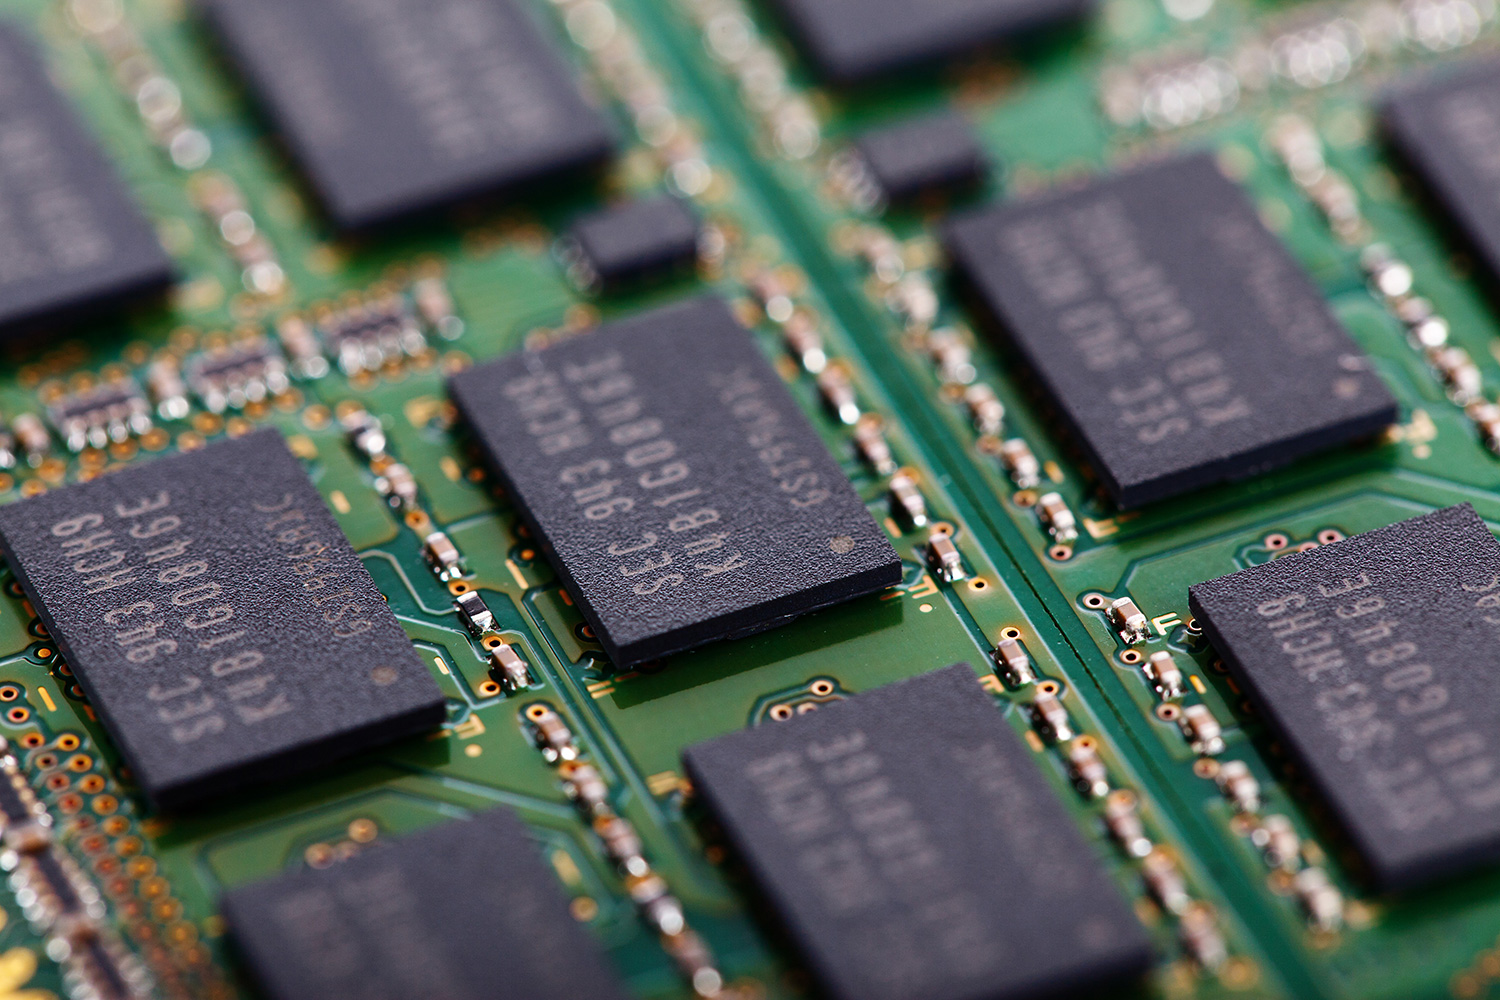
\includegraphics[width=1.00\paperwidth,keepaspectratio]{images/close-up-computer-ram.jpg}}
\begin{frame}[plain]
    \begin{TitleBox}
        \begin{center}
            {\color{red}\Large\inserttitle\color{black}}\\
        \end{center}
        \insertauthor{}\hfill\textbf{\insertinstitute{}}\hfill\insertdate{}\\
        {\footnotesize
        \href{https://hachyderm.io/@tswartz07}{@tswartz07@hachyderm.io}
        \hfill
        \href{mailto: tom@tswartz.net}{tom@tswartz.net}
        }
    \end{TitleBox}
    \vspace{15em}
\end{frame}}

\begin{frame}
  \frametitle{Who is this guy?}
  \framesubtitle{And what is he doing here?}
  \begin{columns}[]
    \begin{column}[T]{0.45\paperwidth}
      {\huge Tom Swartz}
      \vfill
      \begin{itemize}[<+->]
        \item{Crunchy Data \\ Associate Director of Support} 
        \item{Hobbyist interests in `Big Data', IoT, RF Communications}
        \item{I've got some pretty specific hyperfixations}
      \end{itemize}
    \end{column}
    \begin{column}[T]{0.45\paperwidth}
      
\includegraphics[height=4cm,keepaspectratio]{images/logo.png}
    \end{column}
  \end{columns}
\end{frame}

\begin{frame}
  \frametitle{Summary of Applications}
  We'll be reviewing the following topics, and how they relate to Home Automation
  \begin{enumerate}
    \item{Home Assistant}
    \item{ESPHome}
    \item{Building your own Sensors}
  \end{enumerate}
\end{frame}

\section{Home Assistant (and Friends)}
\frame{\sectionpage}

\begin{frame}[fragile]
  \frametitle{Why Home Assistant?}
  \begin{columns}[]
    \begin{column}[T]{0.45\paperwidth}
      \begin{itemize}%[<+->]
        \item{There are a million apps for every `Smart' thing (sometimes multiple for the same item!)}
        \item{A practical application for consolidating software, apps, and tool-sets that many people already use}
        \item{Needs for better usability, security, and maintenance}
        \item{A solid use case for HomeLab equipment, for nerd cred}
     \end{itemize}
    \end{column}
    \begin{column}[T]{0.45\paperwidth}
      
\includegraphics[height=4cm,keepaspectratio]{images/standards.png}
    \end{column}
  \end{columns}
\end{frame}

\subsection{Home Assistant}
\frame{\subsectionpage}

% Install Methods
% Dashboards
% Integrations
% Devices and Entities
% Automations

\section{Security}
\frame{\sectionpage}

\section{Usage and Demo}
\frame{\sectionpage}

% Demo of H-A
% Demo of ESPHome
% Showing ESP Devices in H-A

\section{Custom Sensors}
\frame{\sectionpage}
\subsection{ESPHome}
\frame{\subsectionpage}

% Install methods
% Platforms
% Devices/Components
% Configuration
\subsection{Another Demo}

\section{Wrapping Up}
\frame{\sectionpage}

\begin{frame}
  \frametitle{Key Takeaways}
  \begin{itemize}[<+->]
    \item{Creating your own source of constantly refreshing data for testing purposes is easy, inexpensive, and a great learning experience.}
    \item{If nothing else, you can experiment with a variety of different data sources for PostgreSQL.}
  \end{itemize}
\end{frame}

\begin{frame}[fragile]
  \frametitle{Issues and Lessons Learned}
  \begin{enumerate}
    \item{Great lessons in scripted updates}
    \item{Great use case for data analysis in Postgres}
    \item{Excellent lessons about bulk loading processes}
    \item{Even better lessons in tuning settings for regular large imports}
  \end{enumerate}
\end{frame}

\begin{frame}
  \frametitle{Thank You}
  \begin{center}
    \LARGE{Questions?}
    \vfill
    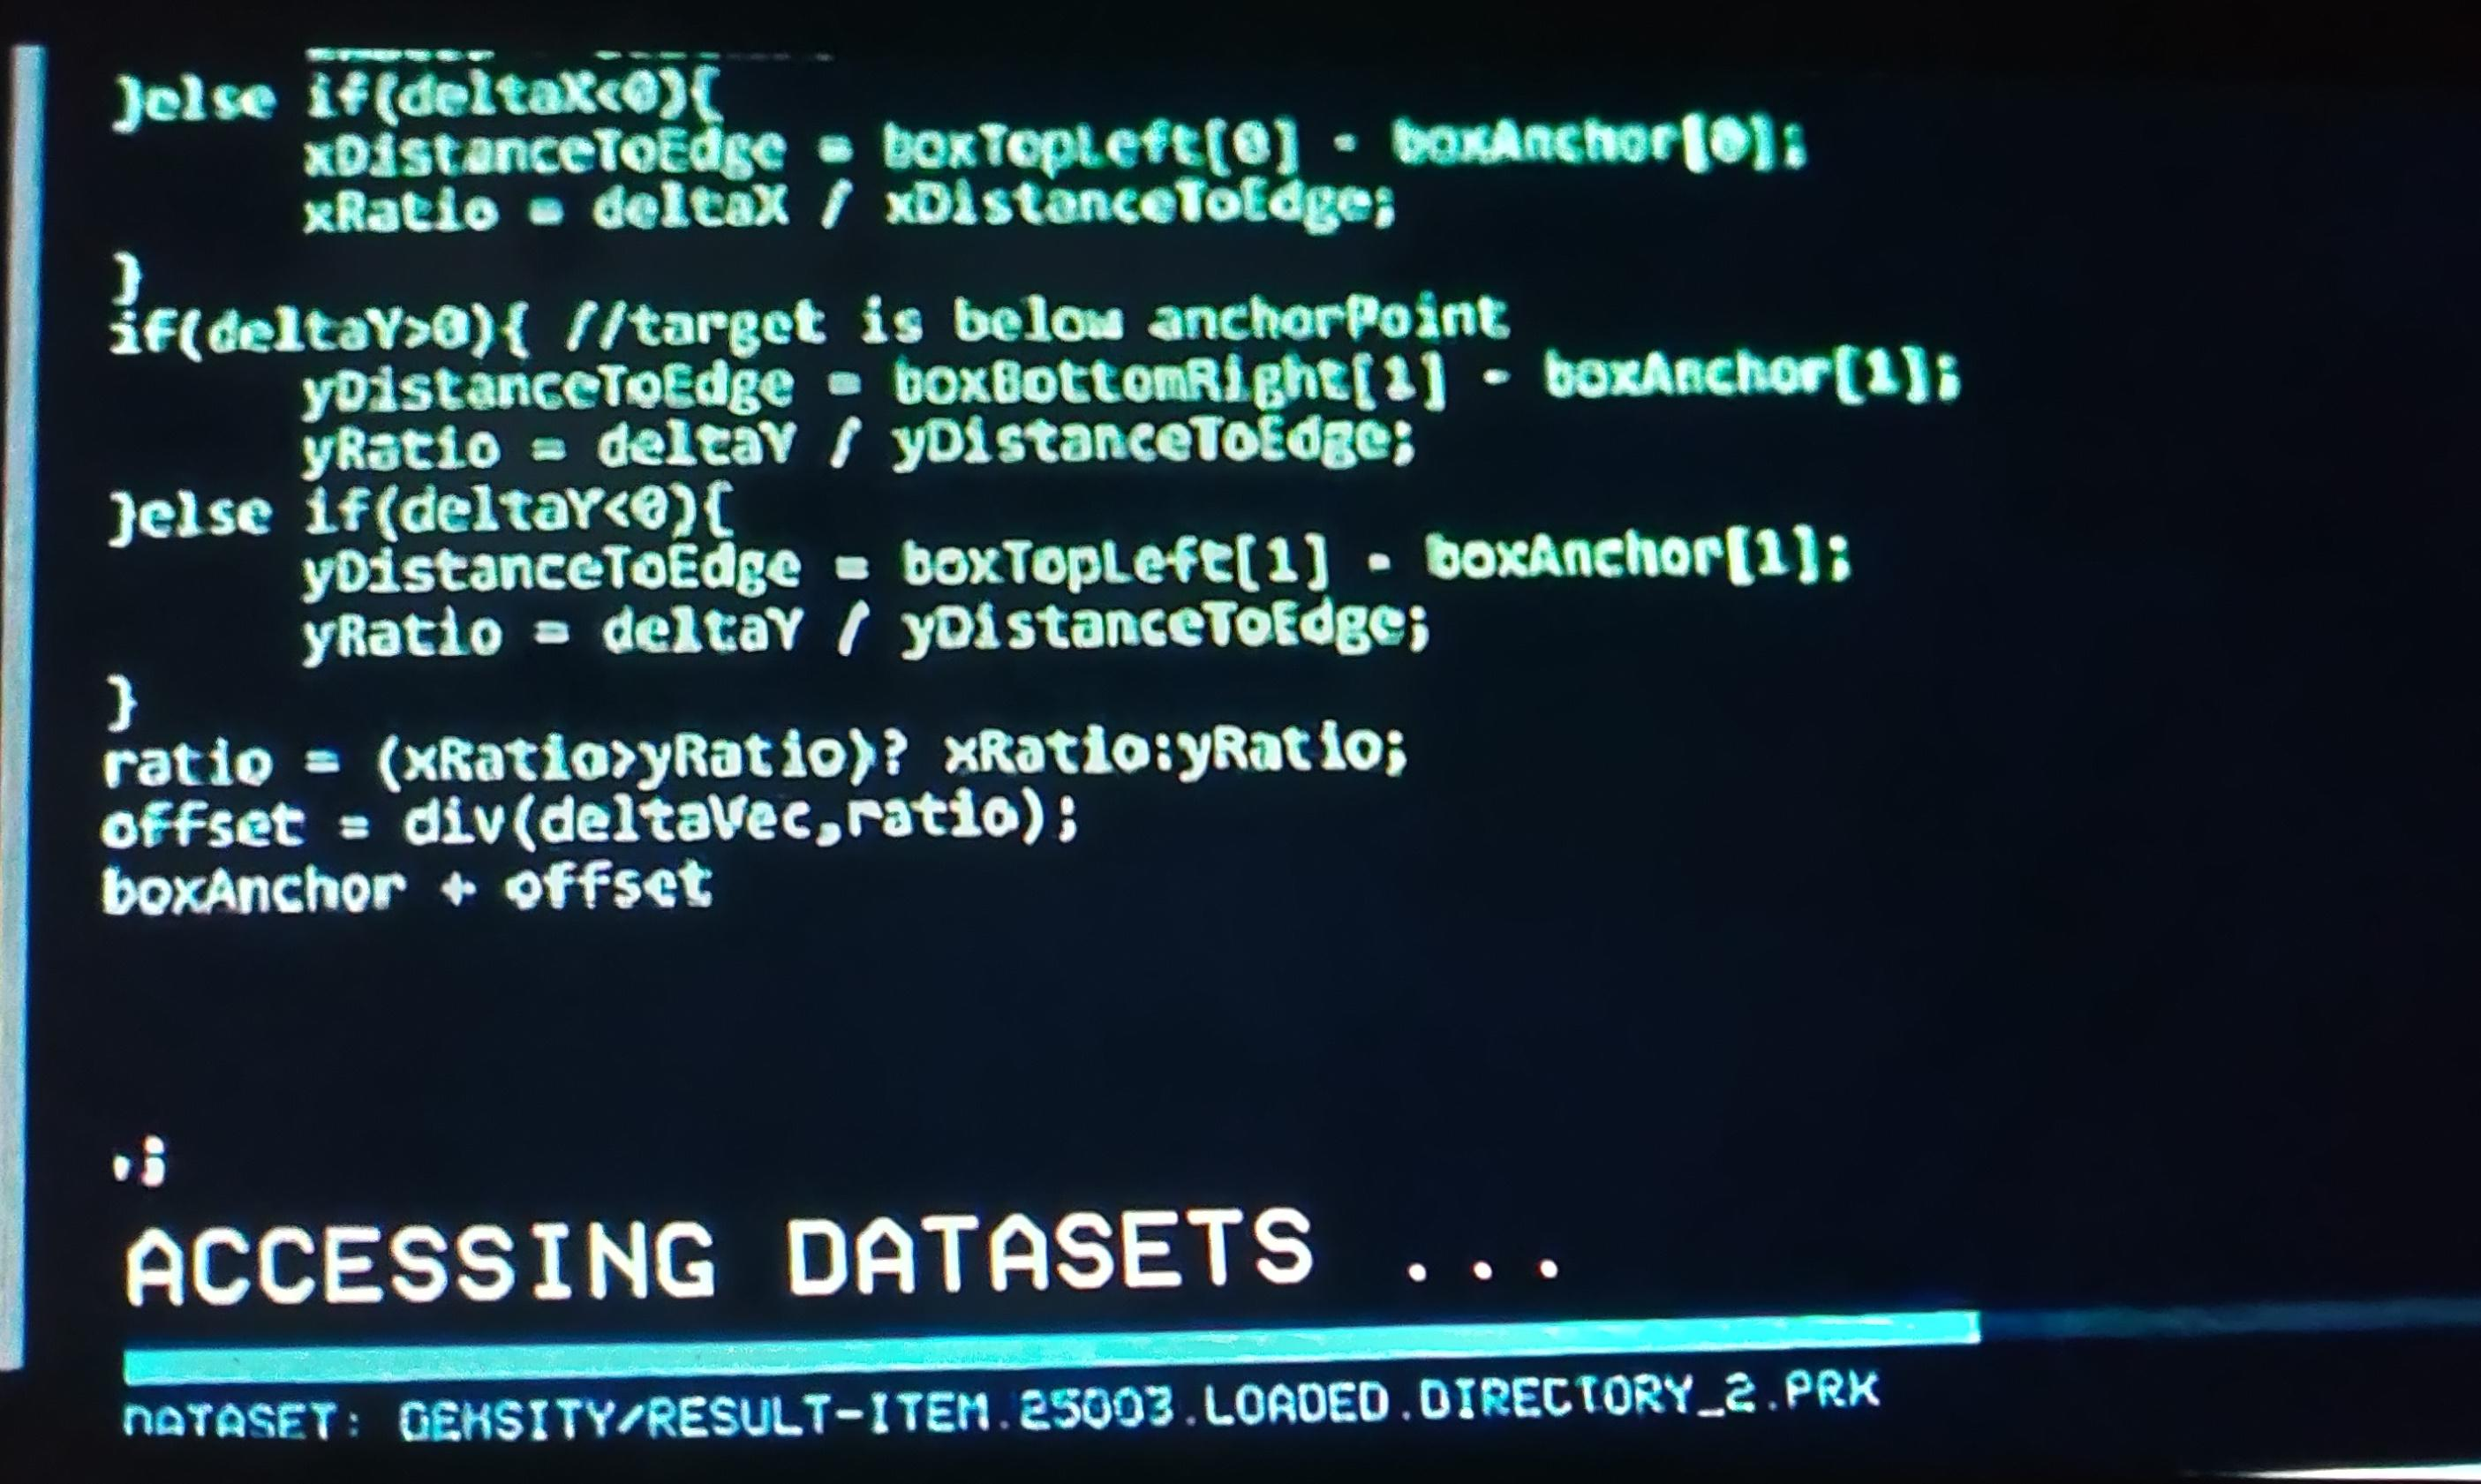
\includegraphics[height=5cm]{images/lol-code.jpg}
  \end{center}
\end{frame}
\begin{frame}[plain,fragile]
  \frametitle{References}
  Code for this presentation, as well as some sample device manifests and other
  information can be found on GitHub and GitLab.
  \begin{itemize}
    \item{\href{https://github.com/tomswartz07/CPOSC2020}{https://github.com/tomswartz07/CPOSC2023}}
    \item{\href{https://gitlab.com/tom.swartz07/CPOSC2020}{https://gitlab.com/tom.swartz07/CPOSC2023}}
  \end{itemize}
  \vfill
  \begin{enumerate}
    \item{\href{https://www.home-assistant.io/}{https://www.home-assistant.io/}}
    \item{\href{https://esphome.io/}{https://esphome.io/}}
    \item{\href{https://www.troyhunt.com/iot-unravelled-part-1-its-a-mess-but-then-theres-home-assistant/}{https://www.troyhunt.com/ IoT Unravelled Series}}
  \end{enumerate}
\end{frame}

\end{document}
% vim: set ts=2 sw=2 spell:
